\RequirePackage{fix-cm}
\documentclass[smallextended]{svjour3}          % twocolumn

\smartqed  % flush right qed marks, e.g. at end of proof

\usepackage{graphicx} % adjustbox loads it
\usepackage{epstopdf} % loads eps
\usepackage[normalem]{ulem}

% insert here the call for the packages your document requires
\usepackage{geometry}
\usepackage[export]{adjustbox}
\usepackage[labelfont=bf, labelsep=space]{caption}
%\usepackage{subcaption}
\usepackage{subfig}
\usepackage[utf8]{inputenc}
\usepackage{amssymb}
\usepackage{amsmath} 

\usepackage{natbib} % enables author year and other citation styles
\usepackage[bookmarks,bookmarksopen,bookmarksdepth=2]{hyperref} % active links
\hypersetup{backref,
	colorlinks=true,
	citecolor=blue,
	linkcolor=blue}

\usepackage{tikz} % graphics,
\usetikzlibrary{fit,positioning} % tikz elements positioning
\usepackage{soul} % annotations


\DeclareMathOperator*{\argmin}{arg\,min}
\DeclareMathOperator*{\argmax}{arg\,max}



\begin{document}

\title{Detection of user roles with thread growth models}
%\subtitle{Do you have a subtitle?\\ If so, write it here}
%\titlerunning{Detection of user roles with thread generative models}        % if too long for running head

\author{Alberto Lumbreras \and
        Julien Velcin  \and\\
        Marie Guégan \and
        Bertrand Jouve
}

%\authorrunning{Short form of author list} % if too long for running head

\institute{Alberto Lumbreras \and Marie Guégan \at
		   Technicolor\\
           975 Avenue des Champs Blancs, \\35576 Cesson-Sévigné,\\ France\\
           \email{alberto.lumbreras@technicolor.com}\\
           \email{marie.guegan@technicolor.com}
           \and
           Julien Velcin \at
           Laboratoire ERIC, Université de Lyon,\\
           5, avenue Pierre Mendès France, 69676 Bron,\\ France\\
           \email{julien.velcin@univ-lyon2.fr}
		  \and
           Bertrand Jouve \at
           Université de Toulouse; UT2; FRAMESPA/IMT; 5 allée Antonio Machado, 31058 Toulouse, cedex 9\\
           CNRS; FRAMESPA; F-31000 Toulouse\\
           CNRS; IMT; F-31000 Toulouse\\ France\\     
           \email{jouve@univ-tlse2.fr}
}

\date{Received: date / Accepted: date}
% The correct dates will be entered by the editor

\maketitle


\section{Introduction}
Random graph models are stochastic generators of graphs that try to reproduce the properties of a some real-world graphs. Ideally, these models should reproduce a large set of properties using a minimum number of assumptions and parameters. If the generated graphs and the real-world graphs share some relevant properties, then the proposed growth mechanism might be a reasonable approximation of the growth laws under which the real-world graphs evolve \citep{Kolaczyk2009}. Formally, a growth model is a probability distribution that quantifies the probability of an existing vertex $i$ of being chosen as the parent for a new vertex $x_t$:
\begin{align*}
p(x_t \sim i | G_{t-1}; \boldsymbol{\theta})
\label{eq:growth_model}
\end{align*} 
where $G_{t-1}$ is the state of the graph before $x_t$ is attached and $\boldsymbol{\theta}$ is the vector of model parameters.

Online discussions can be regarded as evolving tree graphs where vertices represent messages and a directed edge indicates that a message is a reply to another message. The tree starts with the root message that starts the conversation, and then evolves towards some form of tree. Different models have been proposed to account for both the way how a tree evolves and the final properties of the tree. The parameters of these models are fixed and every new vertex is assumed to chose its parent according to the current state of the graph $G_{t-1}$ and a set of fixed parameters that govern the whole process. These parameters regulate, for instance, the tendency to reply to the root, or how fast a vertex with more replies attracts more replies.  Since the parameters are fixed, these models implicitly assume that the choice of a parent is independent of the user who writes the new post.

In this chapter, we explicitly assume that posts written by different users may have different parameters. Some users, for instance, might tend to reply to the root and avoid conversations deeper in the tree. Others might tend to ignore old posts. Others might be specially attracted by popular posts. Formally, we assume that there are $K$ latent types of users and that users of type $k$ behave according to their own group parameters $\boldsymbol{\theta}_k$.  Equation~\ref{eq:growth_model} depends now on the author of post $x_t$:
\begin{align*}
p(x_t \sim i | G_{t-1}; \boldsymbol{\theta}_{z_u})
\end{align*}
where $z_u$ is the group of user $u$ and  $\boldsymbol{\theta}_{z_u}$ are the parameters of that group.

The remaining of this chapters is structure as follows: first, we recall the Preferential Attachment model and we present the thread models. Then we present our model, which finds $k$ sets of parameters for $k$ types of user. Finally, we compare both models and show that, while there is no a remarkable difference on how they reproduce structural properties of real threads, our model can be used for recommendation of posts. 

\section{Network Growth models}\label{sec:related-work}

Growth models try to reproduce not only the final properties of the network but also how the network is built. The \textit{preferential attachment} model proposed by \cite{Barabasi1999} is the best well-known member of this family.
The Barabasi-Albert model builds a graph by sequentially adding its vertices; once a new vertex $x$ is added to the graph it decides whether to create an edge to an existing vertex $i$ with probability

\begin{align}
	p(x \sim i | G) =\frac{d_{i}^\alpha}{Z}; &\qquad
	Z = \sum_{j=1}^{|V(G)|} d_j^\alpha
\end{align}
where $d_i$ is the degree of the vertex $i$ before vertex $x$ is added\footnote{To avoid loaded notations we avoid writing $G_{t-1}$ $d_{i,t-1}$ and $Z_{t-1}$ when it is clear by the context that they correspond to the last state of the graph before adding the new node $x$.}. No This model reproduces a rich-get-richer phenomena controlled by the parameter $\alpha$. The particular case of $\alpha=1$ is called \textit{linear preferential-attachment} since the probabilities increase linearly with the number of degrees. Figure~\ref{fig:Barabasi-Albert} shows examples of Barabasi-Albert graphs generated with different $\alpha$. The Barabasi-Albert explains very well the power-law degree distributions observed in many real graphs.

\begin{figure}
	\centering
	\subfloat[$\alpha=0$]{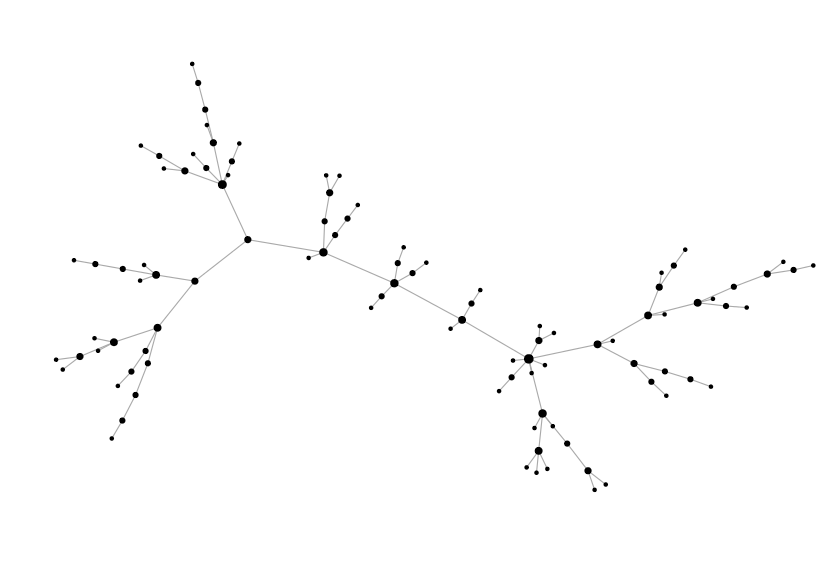
\includegraphics[width=0.33\textwidth]{barabasi_0}}
	\subfloat[$\alpha=1$]{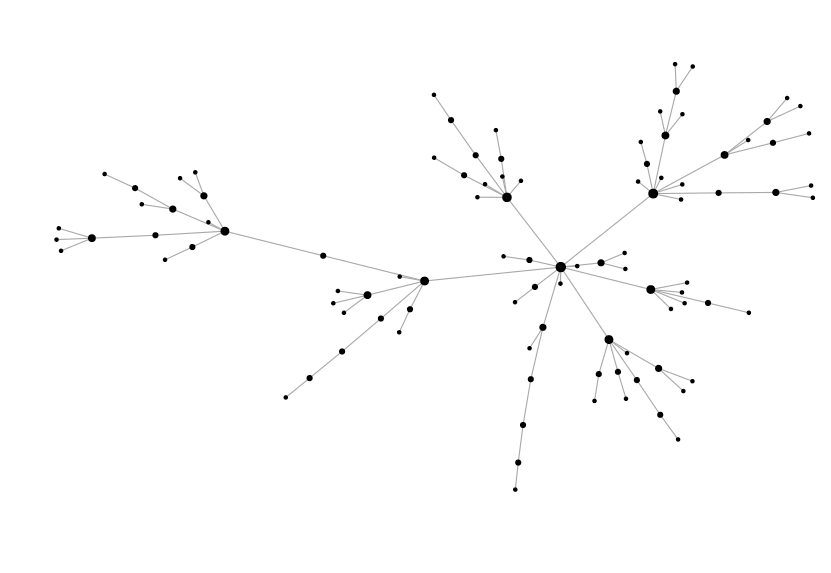
\includegraphics[width=0.33\textwidth]{barabasi_1}}
	\subfloat[$\alpha=1.8$]{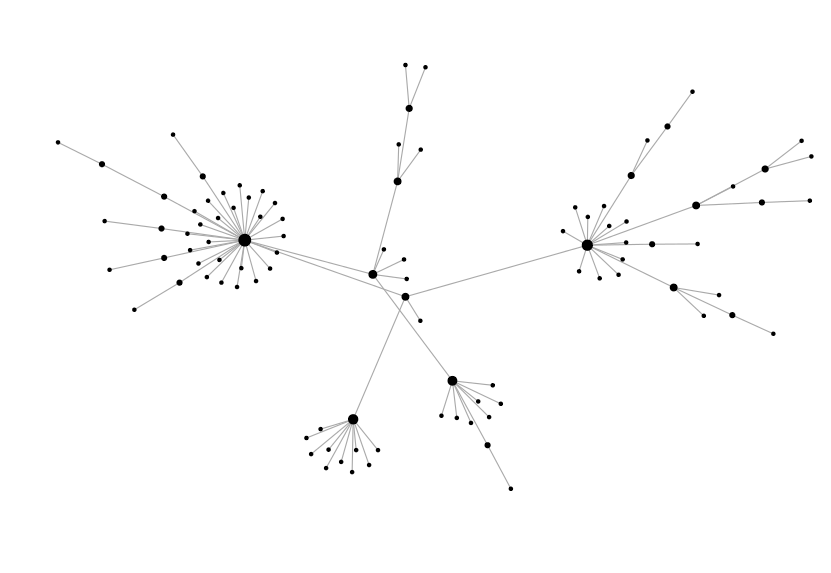
\includegraphics[width=0.33\textwidth]{barabasi_1_8}}
	\caption{Barabasi-Albert graphs with one edge created at every step.}
	\label{fig:Barabasi-Albert}
\end{figure}



In the following sections we describe the growth models that have been proposed to explain the growth of online conversations. A summary is shown in Table X  \citep{Kumar2010, Gomez2010, Wang2012e, Gomez2012}.

\begin{table}
 \begin{center}
   \tabcolsep = 0.8\tabcolsep
   \begin{tabular}{|l|c|l|l|l|}
      \hline
     	 Authors				& $p(x \sim k) \propto$ &Parameters & Estimation & Validation\\
   \hline 
\cite{Barabasi1999} & $d_k^\alpha$  & degree & - &  analytic\\
\cite{Gomez2010} & $(\beta_k d_{k})^{\alpha_k}$ & degree, root & Nelder-Mead & analytic, simulation\\
\cite{Kumar2010} & $\alpha d_k + \tau^{r_k}$ & degree, recency & Grid search &  analytic, simulation \\      
\cite{Gomez2012} & $\beta_k + \alpha d_k + \tau^{t-k}$ & degree, recency, root & Nelder-Mead &  analytic, simulation\\
\cite{Wang2012e} & & &- & -\\
   \hline
   \end{tabular}
\label{tab:growth_models}
 \end{center}
 \caption{Growth models for online discussions}
\end{table}
%\end{figure}

%%%%%%%%%%%%%%%%%%%%%%%%%%%%
\subsection{Kumar model}
\cite{Kumar2010} proposed a model that combines both \textit{preferential-attachment} and \textit{recency}. The higher the degree of a post and the later it was published, the easier for this post to attract the incoming replies. At every time step, a decision is made to stop the thread or to add a new post. Every new post choses its parent according to:
\begin{align}
p(x\sim i | G) = \frac{h(d_k, r_k)}{Z}; \qquad h(d_k, r_k) =\alpha d_k + \tau^{r_k} ; \qquad Z = \sum_{n=1}^{|V(G)|} h(d_n, r_n) + \delta
\end{align}
and the probability of stopping the thread is:
\begin{align}
p(x\sim i | G) = \frac{\alpha}{Z}; 
\end{align}



where $r_u$ is the number of time steps since $u$ was added to the thread. The authors report that when the alternative function $h(d_u, r_u) = d_u \tau^{r_u}$ is used, the recency factor prevents the preferential attachment factor from generating heavy-tailed degree distributions. The choice of placing $\alpha$ as a coefficient instead of an exponent is made for mathematical convenience so that $Z$ does not depend on the graph structure at that particular moment. The function of the $delta$ in the denominator is to give some probability to the death of the discussion. 

The authors also propose an improvement of the model to account for the identity of posts authors. For a new post $v$ replying to a post $u$, its author $a(v)$ can be either $a(u)$ (a self-reply), another author $a(w)$ that has already participated in the chain from $u$ to the root, or some other new author belonging to the set of authors $A$ that have not participated in the chain:
\begin{align}
a(v) = 
\begin{cases}
a(w) & \text{ with probability } \gamma\\
a(u) & \text{ with probability } \epsilon\\
a \in A & \text{ with probability } 1 -\gamma - \epsilon 
\end{cases}
\end{align} 

The Maximum Likelihood Estimators of the parameters $\alpha, \tau, \gamma, \epsilon$ are found by a grid search.

\subsection{Gomez model (2010)}
In \cite{Gomez2010} the authors combine \textit{preferential-attachment} with a \textit{bias towards the root}. The probability of choosing an existing parent $k$ is:
\[
%p(\pi_t = k | \boldmath{\pi}_{(1:t-1)}) 
%\propto 
%(\beta_k d_{k,(t-1)})^{\alpha_k}
p(x \sim k | G) 
\propto 
(\beta_k d_{k})^{\alpha_k}
\]
where 
\begin{align}
\alpha_k = 
\begin{cases}
	\alpha_1 & \text{ for } k=1 \\	
	\alpha_c & \text{for } k \in \{2,...,t\}
\end{cases}\notag\\
\beta_k = 
\begin{cases}
\beta & \text{ for } k=1 \\	
1 & \text{for } k \in \{2,...,t\}
\end{cases}
\end{align}
Note that $\alpha_k$ is the preferential attachment exponent and that if $\alpha_1=\alpha_c$ and $\beta=1$ we recover the Barabasi-Albert model of preferential attachment.

The Maximum Likelihood Estimators of the parameters $\alpha, \tau, \gamma, \epsilon$ are found using the loglikelihood:

%\begin{equation}
%	\log \mathcal{L}(\boldsymbol{\Pi} | \alpha_k, \beta_k)
%	=
%	\sum_{i=1}^{N}
%	\sum_{t=2}^{|\pi_i|}
%	\alpha_k (\log \beta_k+ \log d_{k,1:(t-1)}) 
%	-
%	\log \sum_{l=1}^{t} (\beta_l d_{l,1:(t-1)})
%\end{equation}
\begin{equation}
\log \mathcal{L}(\mathbf{G} | \alpha_k, \beta_k)
=
\sum_{i=1}^{N}
\sum_{t=2}^{|V(G_i|}
\alpha_k (\log \beta_k+ \log d_{k,(t-1)}) 
-
\log \sum_{l=1}^{t} (\beta_l d_{l,(t-1)})
\end{equation}
The minimization is done with the Nelder-Mead algorithm (\texttt{fminsearch} in Matlab). Though Nelder-Mead can be used in non-convex functions, this loglikelihood is convex. Parameters are fitted to the dataset under study and then we generate graphs that resemble the original conversations (see Figure~\ref{fig:Gomez}).

	\begin{figure}
		\centering
		\subfloat[real]{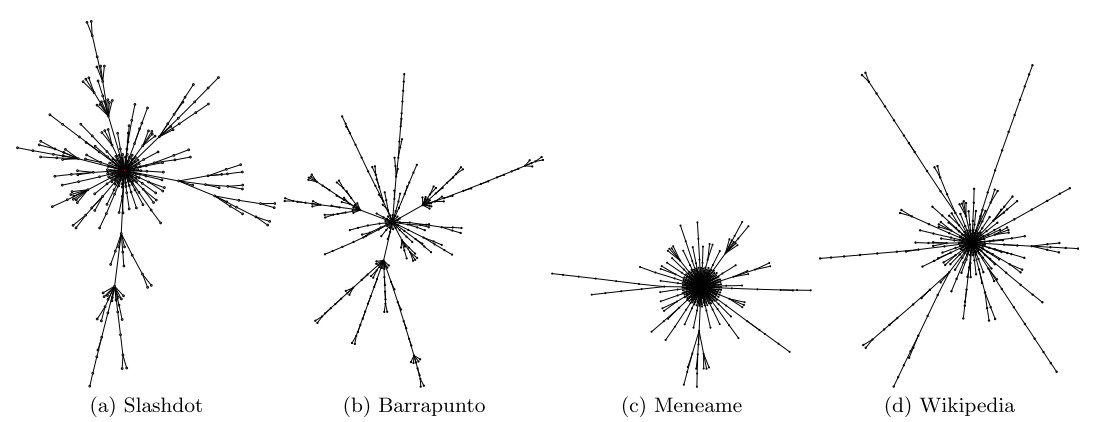
\includegraphics[width=0.45\textwidth]{gomez_real}}\hfill
		\subfloat[synthetic]{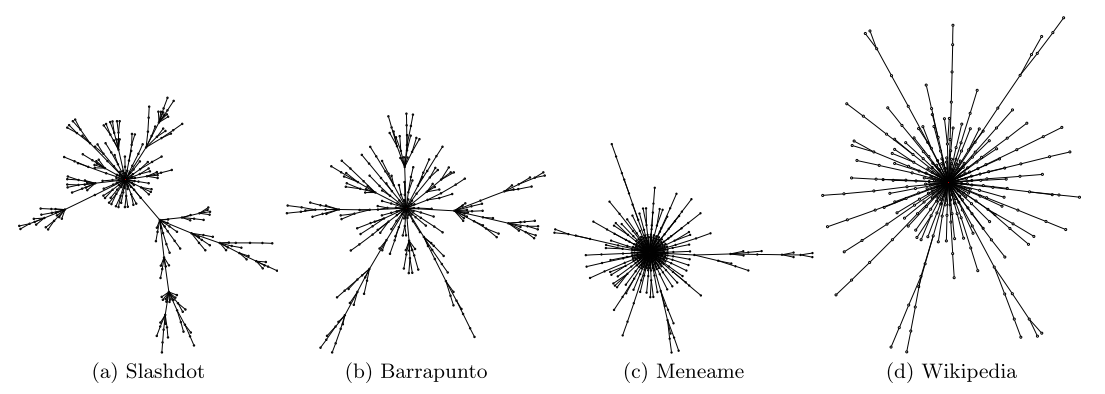
\includegraphics[width=0.45\textwidth]{gomez_synthetic}}
		\caption{Random grahs for discussion threads. Gómez-Kappen-Kaltenbrunner}
		\label{fig:Gomez}
	\end{figure}

\subsection{Gomez model (2012)}
In \cite{Gomez2012} the authors combine \textit{preferential-attachment}, a \textit{bias towards the root} and \textit{novelty}. Unlike in their former model in \cite{Gomez2010}, here they sum these factors instead of multiplying them:

\begin{equation}
%p(\pi_t = k | \boldmath{\pi}_{(1:t-1)}) 
%\propto 
%(\beta_k d_{k,(t-1)})^{\alpha_k}
p(x \sim k | G) 
\propto 
\beta_k + \alpha d_{k, (t-1)} + \tau^{t-k}
\end{equation}

The negative log-likelihood to be minimized is: 
\begin{equation}
\log \mathcal{L}(\mathbf{G} | \alpha, \beta_k, \tau)
=
\sum_{i=1}^{N}
\sum_{t=2}^{|V(G_i)|}
\log
\left(
\beta_k+
\alpha d_{k,(t-1)}
+ \tau^{t-k}
\right)
- \log
\sum_{l=1}^{t}
\left(\beta_l+
\alpha d_{l, (t-1)}
+ \tau^{t-l}
\right)
\end{equation}
As in \cite{Gomez2010}, Maximum Likelihood Estimators are found by Nelder-Mead optimization. Unlike their previous model, this loglikelihood is non-convex. Authors reported that, for large enough data, the optimization algorithm tends to give the same optimum for different initialization.



\subsection{Wang model}

%\subsection{Time-sensitive preferential attachment}
In \cite{Wang2012e} authors make two observations. On the one hand, that distance between its posts follows an upper-truncated Pareto distribution. On the other hand, that threads grow faster when they are featured in the front page (or some sections showing the top discussions at that moment) and they slow down once they disappear from the front page. From this, they propose a model that models the growth of a thread in a given forum. As for the structure, they use preferential-attachment. It is the only existing model that includes real time.

\subsubsection*{Parameter estimation}
Their model has two parts: a upper-truncated distribution to model the time of response and the preferential attachment to model the structure.
Authors use their Maximum Likelihood estimators, which are both known in the literature.

\subsection{Limitations of current models}
There are two aspects that might me improved:

\begin{itemize}
	\item Time is only poorly combined with the structure in \cite{Wang2012e}. Actually in this model time is independent of the structure and vicecersa. As suggested in \cite{Gomez2012} (Conclusions) combining both time and structure is an interesting line of research. Besides, there are probably other ways of consider time.
	
	\item These models estimate their parameters once and therefore very different threads are summarized with common parameters. However, imagine that we learned our parameters from a set of threads $\mathbf{G}$ and now we want to make predictions on a particular new thread $G^*$, that is, we want to compute $p(x \sim i | G_{1:t-1}^*, \mathbf{G})$. There is a lot to be learned from the particular ongoing dynamics of the conversation until time $t$, and making predictions based on the globally estimated parameters will not be flexible enough to adapt the prediction to the last observations. Bayesian inference is a natural way to do this since we will be constantly updating our believes every time a new observation (post) arrives. The challenge here is its computational cost, so we should probably work with fast approximations to the posterior

	\item Current models consider that the likelihood of choosing a parent is independent on the user who writes the post. In other words, that the model parameters are shared by all the users. However, it seems reasonable to think that different users may behave according to different parameters (e.g.: different attraction towards the root or towards popular posts).
\end{itemize}

In the following section, we present a modification to the model of \citep{Gomez2012} that finds different parameters for different groups of users. We also analyse whether this feature can improve the model when used for a task of post recommendation. 

\section{A mixture-based model}
For any given post $n$, let $d_n$ denote the degree of its parent; let $r_n$ be 1 if the parent of $n$ is the root, and 0 otherwise. Let $l_n$ be the number of time steps elapsed between the parent of $n$ and $n$ ($l_n \geq 1$). Let $\mathbf{X} = \{\mathbf{x}_1,...,\mathbf{x}_N\}$ be the set of posts and let $\mathbf{x}_i = \{t_i, d_i, r_i, l_i\}$  be the set of features associated to a post. Let us assume that there are there are $K$ different types, or roles, of users that behave following different parameters $\boldsymbol{\theta}_1$,...,$\boldsymbol{\theta}_K$ where  $\boldsymbol{\theta}_k = \{\alpha_k, \beta_k, \tau_k$\}. Let $z_u$ be the role of user $u$. Let $N_u$ be de set of posts written by $u$. The likelihood can be expressed as:
\begin{align}
\ln p(\mathbf{X} | \boldsymbol{\theta}) = 
\sum_{u=1}^U \sum_{n \in N_u} 
\frac{1}{Z_n}\left(\alpha_{z_u} d_{n} + \beta_{z_u}r_{n} + \tau_{z_u}^{l_n}\right)
\end{align}
where $Z_n$ is a normalization factor that guarantees that the probabilities of all possible choices sum up to one. Let $t$ be the number of time steps between the root and the post $n$. The normalization factor is computed for every new post as:

\begin{align*}
Z_n &=  
\sum_{m | t_m < t_n} \alpha_{z_m} d_m + \beta_{z_m} r_m + \tau_{z_m}^{l_m} \qquad\text{for $m$ in same thread than $n$}
\\&=
\alpha_{z_m}(2t -1) + \beta_{z_m} + \frac{\tau_{z_m}(\tau_{z_m}^t-1)}{\tau_{z_m}-1}
\end{align*}
where $z_m$ denote the cluster of the user who wrote the post $m$. Note that this sum does not depend on the structure of the discussion.

\subsection{Expectation-Maximization} 
We want to estimate the parameters of each role $\boldsymbol{\theta}_1,...,\boldsymbol{\theta}_K$ and the latent role of every user $z_1,...,z_U$. If there was one one group of $\boldsymbol{\theta}$ there would be no $\mathbf{Z}$ and we could use Nelder-Mead to find the parameters. However, if there are different groups then the optimization of the parameter will depend on the group since the parameters will be optimized considering who belongs to that group. This is a classic scenario that can be solved by Expectation Maximization (EM). In EM, we do an iterative optimization over the parameters $\boldsymbol{\theta}_1,...,\boldsymbol{\theta}_K$ and the class assignments $\boldsymbol{z}_1,...,\boldsymbol{z}_U$ until the likelihood converges. In particular, we maximize a lower bound of the loglikelihood:
\begin{align}
\ln p(\mathbf{X} | \boldsymbol{\theta}) 
\leq
\overbrace{
\underbrace{
\sum_{\mathbf{Z}} q(\mathbf{Z})\ln p(\mathbf{X, \mathbf{Z} | \boldsymbol{\theta}})
}_{\mathbb{E}_\mathbf{Z}\left[\ln p(\mathbf{X, \mathbf{Z} | \boldsymbol{\theta}})\right]} 
-
\underbrace{
\sum_{\mathbf{Z}}
q(\mathbf{Z}) 
\ln q(\mathbf{Z})
}_{entropy~H(\mathbf{Z})}
}^{\mathcal{L}(q, \boldsymbol{\theta})}
\end{align}
where $q$ is some arbitrary probability distribution. The EM algorithm starts by some initial values of $\boldsymbol{\theta}$. In the E-step, we adjust the function $q(\mathbf{Z})$ so that it maximizes the lower bound assuming that the parameters are fixed. This happens when $q(\mathbf{Z})$ is the posterior:
\begin{align}
q(\mathbf{Z}) = p(\mathbf{Z} | \mathbf{X}, \boldsymbol{\theta}) 
\end{align}
Moreover, in that case the lower bound $\mathcal{L}(q,\boldsymbol{\theta})$ reaches the true loglikelihood $\ln p(\boldsymbol{X} | \boldsymbol{\theta})$. In the M-step we optimize the lower bound with respect to the parameters. We will now make the $\boldsymbol{\pi}$ parameters of the prior distribution $p(\mathbf{Z} | \boldsymbol{\pi})$ explicit. Since we fixed $q(\mathbf{Z})$, the entropy term is constant, and thus we just have to maximize the first term. After we plug-in the recently computed $q(\mathbf{Z})$ and using the chain rule, we obtain:
\begin{align*}
\argmax_{\boldsymbol{\theta}, \boldsymbol{\pi}} 
\underbrace{
\sum_{\mathbf{Z}} p(\mathbf{Z} | \mathbf{X}, \boldsymbol{\theta})
\overbrace{
\left(\ln p(\mathbf{Z} | \boldsymbol{\pi})  + \ln p(\mathbf{X  | \mathbf{Z}, \boldsymbol{\theta}})\right)
}^{\ln p(\mathbf{X}, \mathbf{Z} | \boldsymbol{\theta})}
}_{\mathbb{E}_\mathbf{Z}\left[\ln p(\mathbf{X, \mathbf{Z} | \boldsymbol{\theta}})\right]} 
\end{align*}

We repeat the E and the M step until the improvement in the likelihood is lower than some threshold $\epsilon$.

\subsection{EM for the random threads model}
In this section we provide the exact equations to maximize in the E and M steps for our model.
Let $\mathbf{X}_u$ the submatrix of $\mathbf{X}$ composed of all posts written by user $u$. Let $\mathbf{Z} = \{\mathbf{z}_1,...,\mathbf{z}_U\}$ be the indicators matrix where $\mathbf{z}_i=\{z_{i1},...,z_{iK}\}$ and where $z_{ik}$ is one if user $i$ belongs to group $k$ and zero otherwise. For, the M-step, the expectation of the complete loglikelhood is:
\begin{align}
\mathbb{E}\left[
\ln p(\mathbf{X, Z} | \boldsymbol{\theta}) 
\right]
&= 
\mathbb{E}\left[
\sum_{u=1}^U 
\sum_{k=1}^K 
z_{uk}
\left\lbrace\ln \pi_k + 
\ln p(\mathbf{X}_u | \boldsymbol{\theta}_k)\right\rbrace
\right]
=
\sum_{k=1}^K 
\sum_{u=1}^U 
\mathbb{E}\left[z_{uk}\right]
\left\lbrace
\ln \pi_k + 
\ln p(\mathbf{X}_u | \boldsymbol{\theta}_k)
\right\rbrace
\label{eq:m-step}
\end{align}
where, for a given cluster $k$, each $\mathbf{X}_u$ contributions proportionally to $\mathtt{E}[z_{uk}]$ being considered are those of users that belong to that cluster. In the E-step we update the posterior
\begin{align}
p(\mathbf{Z} | \mathbf{X},\boldsymbol{\theta})
=
\frac{
p(\mathbf{X}, \mathbf{Z} | \boldsymbol{\theta})
}
{
\sum_{\mathbf{Z}} p(\mathbf{X}, \mathbf{Z} | \boldsymbol{\theta})
}
=
\frac
{\prod_{u=1}^U\prod_{k=1}^K  p(\mathbf{X}_u | \boldsymbol{\theta}_k)^{z_{uk}}}
{\sum_{\mathbf{Z}} \prod_{u=1}^U\prod_{k=1}^K  p(\mathbf{X}_u | \boldsymbol{\theta}_k)^{z_{uk}}}
\end{align}
which can be easily factorized by users, and then we can obtain the expected value for each $z_{uk}$:
\begin{align}
\mathbb{E}[z_{uk}] 
=
\sum_{z_{uk}} z_{uk} 
\frac
{\pi_k p(\mathbf{X}_u | \boldsymbol{\theta}_k)}
{\sum_{k=1}^K \pi_k p(\mathbf{X}_u | \boldsymbol{\theta}_k)}
=
\frac
{\pi_k p(\mathbf{X}_u | \boldsymbol{\theta}_k)}
{\sum_{k=1}^K \pi_k p(\mathbf{X}_u | \boldsymbol{\theta}_k)}
\label{eq:e-step}
\end{align}
where the likelihood $p(\mathbf{X}_u | \boldsymbol{\theta}_k)$ can be also factorised:
\begin{align}
   p(\mathbf{X}_u | \boldsymbol{\theta}_k) = \prod_{n \in N_u} p(\mathbf{x}_n | \boldsymbol{\theta}_k)
\end{align}

The E-step is done with Equation~\ref{eq:e-step} and the M-step is done with Equation~\ref{eq:m-step} Since due to the form of our likelihood the equation cannot be analytically maximized, we use Nelder-Mead optimization.

\subsection{Number of clusters}
\section{Experiments}
In this section, we validate our model for two different tasks. First, we analyse whether our model explain some structural properties of discussion threads better than \cite{Gomez2012}. Second, we compare both models for the task of recommending a post to a user than joins the discussion. We do all our experiments in two Reddit forums: \texttt{podemos} and \texttt{gameofthrones}.

\subsection{Reproduction of structural properties} 
For each dataset, we estimated the parameters of \citep{Gomez2012} and our model. Then, we generated artificial threads and measured the following properties:

\begin{itemize}
\item degree distribution
\item subtree size
\item size versus depth
\item width versus depth
\end{itemize} 

\begin{figure}
\center
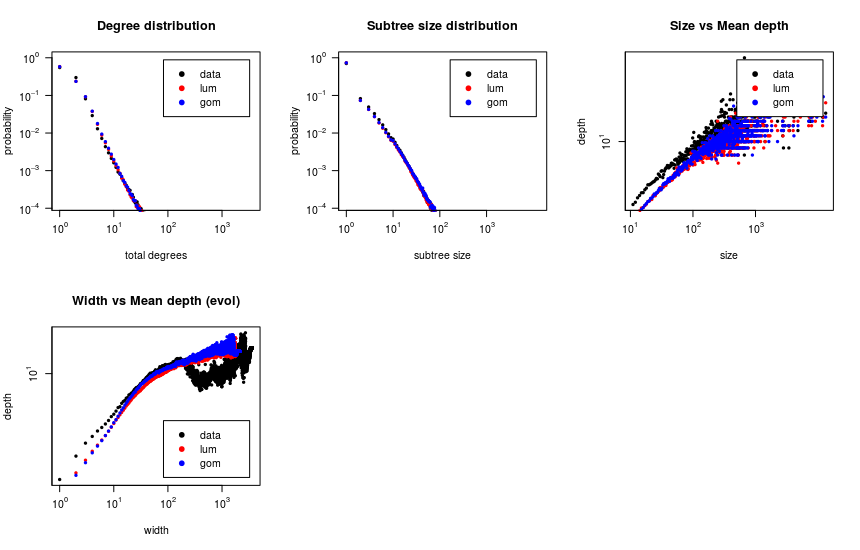
\includegraphics[width=1\textwidth]{benchmark_structures_gof}
\caption{Synthetic trees vs real trees in Game of Thrones}
\end{figure}
\begin{figure}
\center
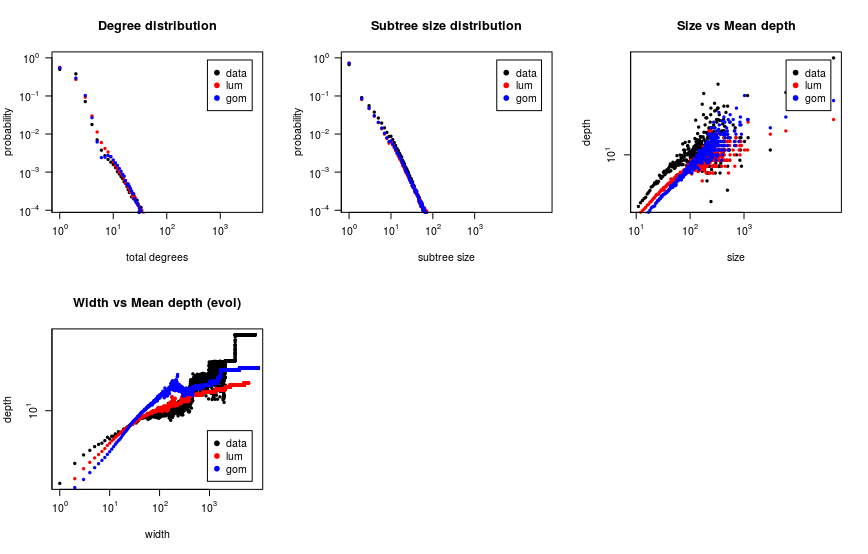
\includegraphics[width=1\textwidth]{benchmark_structures_podemos}
\caption{Synthetic trees vs real trees in Podemos}
\end{figure}

\subsection{Recommendation of posts}
Assuming that we know that a new user is going to participate in the discussion, the recommendation task is to predict to which posts he will reply, taking the one with more probability according to our likelihood function and the estimated parameters:
\begin{align*}
\argmax_k p(x \sim k)
\end{align*}
Surprisingly, the post with the maximum likelihood is always the root.


\begin{figure}
\center
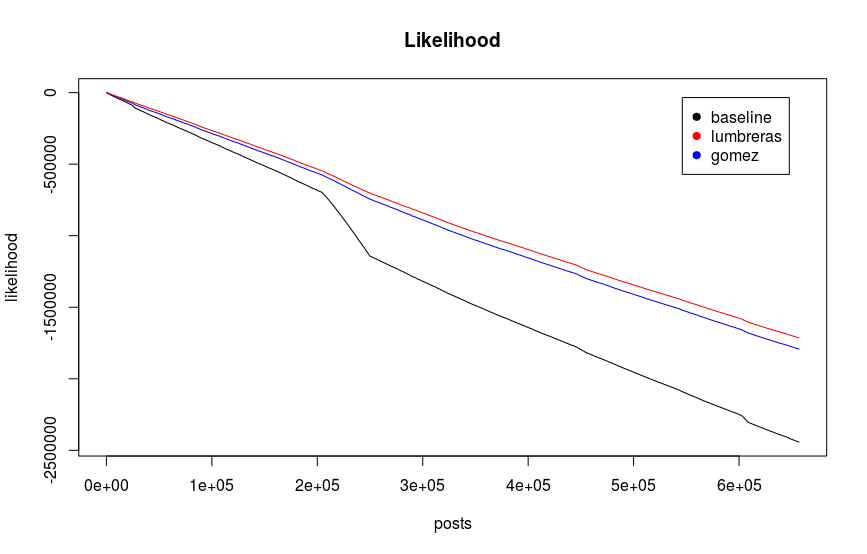
\includegraphics[width=1\textwidth]{predictions_likelihood_podemos}
\caption{Likelihood of post parents according two different models (Podemos)}
\end{figure}

\begin{figure}
\center
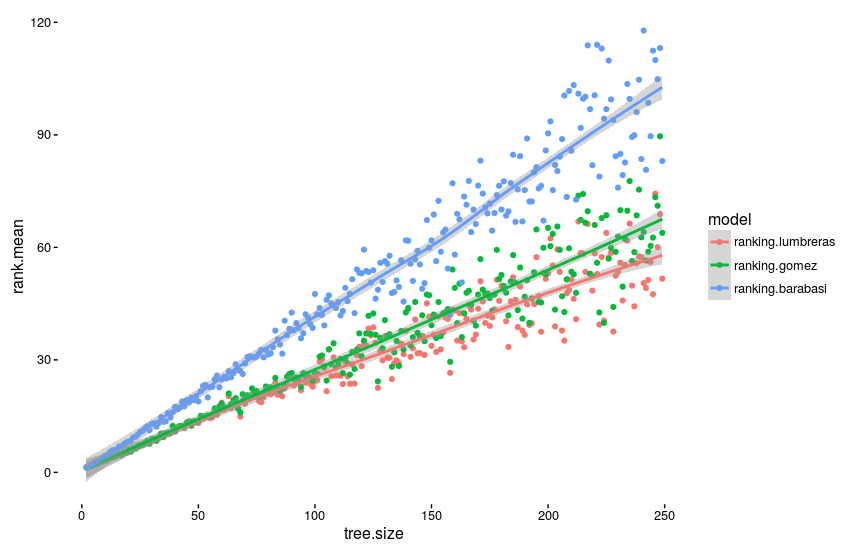
\includegraphics[width=1\textwidth]{benchmark_ranking}
\caption{Likelihood of post parents according two different models (Podemos)}
\end{figure}


\newpage
\appendix
\section*{Appendices}
\section{Expectation-Maximization}

\begin{align}
\ln p(\mathbf{X} | \boldsymbol{\theta}) &=  \ln \sum_{\mathbf{Z}}  p(\mathbf{X}, \mathbf{Z}  | \boldsymbol{\theta}) \\
&=\ln \sum_{\mathbf{Z}} q(\mathbf{Z}) \frac{p(\mathbf{X}, \mathbf{Z}  | \boldsymbol{\theta})}{ q(\mathbf{Z})}\\
&\geq \sum_{\mathbf{Z}} q(\mathbf{Z}) \ln \frac{p(\mathbf{X}, \mathbf{Z} | \boldsymbol{\theta)}}{q(\mathbf{Z})}
\end{align}


The equality holds when $q(\mathbf{Z})$ is the posterior $p(\mathbf{Z} | \mathbf{X}, \boldsymbol{\theta})$:
\begin{align}
\ln p(\mathbf{X} | \boldsymbol{\theta}) &=  \sum_{\mathbf{Z}} p(\mathbf{Z} | \mathbf{X}, \boldsymbol{\theta}) \ln \frac{p(\mathbf{X, Z} | \boldsymbol{\theta})}{ p(\mathbf{Z} | \mathbf{X}, \boldsymbol{\theta})} \qquad \blacksquare
\label{eq:em_general}
\end{align}
%\bibliographystyle{chicago} % or plain
\bibliographystyle{spbasic} 
\bibliography{bibliography}
\end{document}